%% Manuscript for The Journal of the Astronautical Sciences (Springer Nature LaTeX template, sn-jnl).
%% Build:  pdflatex main && bibtex main && pdflatex main && pdflatex main
%% Figures: figures/jas/Fig1.pdf ... Fig16.pdf (vector) and Fig*.tif (600 dpi) from the scripts.
\documentclass[pdflatex,sn-mathphys-num]{sn-jnl}

\usepackage{graphicx}
\usepackage{multirow}
\usepackage{amsmath,amssymb,amsfonts}
\usepackage{bm}
\usepackage{booktabs}
\usepackage{xcolor}
\usepackage{textcomp}
\usepackage{manyfoot}
\usepackage{orcidlink}
\graphicspath{{../figures/jas/}}

\newcommand{\Tc}{T_{\mathrm{c}}}
\newcommand{\vect}[1]{\bm{#1}}

\raggedbottom

\begin{document}

\title[Custody Horizons for Ground-Based Cislunar Tracking]{Custody Horizons for Ground-Based Angles-Only Tracking of Cislunar Periodic Orbits}

\author*[1]{\fnm{Bishwaswarup} \sur{Nayak}\,\orcidlink{0009-0001-9926-5329}}\email{bishwaswarup@iisc.ac.in}

\affil*[1]{\orgdiv{Department of Physics}, \orgname{Indian Institute of Science}, \orgaddress{\city{Bengaluru}, \postcode{560012}, \state{Karnataka}, \country{India}}}

\abstract{Ground-based telescopes lose cislunar objects for days at a time. This paper quantifies the custody horizon: how long an object on a cislunar
periodic orbit can go unobserved before it leaves a telescope search pattern centred on the operator's
own unscented-transform prediction. Four Earth--Moon orbits (the 9:2 near-rectilinear halo
orbit, an $L_1$ halo, an $L_2$ Lyapunov orbit and a distant retrograde orbit) are observed for one
year by a simulated four-site network of 1\,m telescopes. The targets stay within 14$^\circ$ of the
Moon, so the Moon-exclusion angle matters more than aperture, and the longest lunar-phase blackout
lasts 8.5--15.7\,days. After a 3-day gap on the $L_1$ halo, the extended Kalman filter reacquires
consistently in 37\,\% of 100 runs, against 100\,\% for a Gaussian-mixture unscented filter. The
operator horizon equals that of an idealised search centred on the true mean (median ratio 1.00). The
near-rectilinear and distant retrograde orbits stay in custody beyond 30\,days after three or more
days of tracking, whereas the unstable $L_1$ and $L_2$ orbits are lost after 11--17\,days (median,
ten fields), depending mainly on the tracking-arc length. Across 30 members of five families, the
horizon falls with the stability index (Spearman $\rho = -0.92$ above index 10). Individual horizons
are predicted by the unscented-transform covariance, not by the finite-time Lyapunov exponent. Site biases and
solar-pressure errors shorten the horizons by about 1\,\% at nominal levels but make covariance-based
custody claims overconfident. The main conclusions are reproduced for 60 cases in a DE440 ephemeris model with solar radiation pressure.}

\keywords{Cislunar space domain awareness, Angles-only orbit determination, Near-rectilinear halo orbit,
Uncertainty propagation, Gaussian mixture filter, Custody}

\maketitle

%=====================================================================
\section{Introduction}\label{sec:intro}

Traffic beyond geosynchronous orbit is growing: lunar orbiters, the Gateway's 9:2
near-rectilinear halo orbit (NRHO), and spacecraft in libration-point and distant retrograde
orbits (DROs). Keeping track of these objects, that is, maintaining \emph{custody}, is harder than
in near-Earth space for three reasons. The targets are faint and about 380\,000\,km away. Seen from
Earth, they sit close to the brightest object in the night sky. And their motion is governed by
the Earth--Moon three-body problem, which stretches uncertainty rapidly and makes it
non-Gaussian~\cite{frueh2021}.

Ground-based optical telescopes are the most accessible sensors for this task.
Sechrest et al.~\cite{sechrest2024} detected CAPSTONE at $g \approx 19.6$ and Orion at
$g \approx 15.5$ with 36\,cm telescopes. But ground sensors see cislunar objects only
intermittently: daylight, the Moon's glare and the lunar phase open and close observation windows.
Earlier work has shown that filters survive or fail across particular gaps on particular
trajectories~\cite{chow2021,chow2022,iannamorelli2023}. What is missing is a systematic answer, at least for representative orbits, to
the operational question: \emph{how long can a cislunar object go unobserved before it cannot be found
again, and what determines that time?}

This paper answers that question for ground-based, angles-only tracking of periodic orbits in a
simulation study. Its contributions are:
\begin{enumerate}
\item A physically generated observation model (sites, twilight, Moon exclusion and occultation,
      shadows, photometry with scattered moonlight). It shows that the targets studied stay within
      14$^\circ$ of the Moon and that monthly lunar-phase blackouts of up to two weeks cannot be
      removed by adding ground sites (Section~\ref{sec:vis}).
\item A definition of the \emph{custody horizon} $\Tc$ as the longest gap after which 99\,\% of the
      true probability mass still lies inside a telescope search pattern, and maps of $\Tc$ across
      orbits, tracking-arc lengths and search sizes for a search centred on the operator's own
      unscented prediction, which keeps custody as long as an idealised search centred on the truth
      (Section~\ref{sec:custody}).
\item Evidence that $\Tc$ can be predicted without Monte Carlo from the propagated post-fit
      covariance (unscented transform), but not from the orbit's finite-time Lyapunov exponent
      alone (Section~\ref{sec:predict}).
\item A quantification of when the filter choice matters: linear (extended Kalman filter)
      prediction gives false custody on unstable orbits after long gaps, and a Gaussian-mixture
      filter reacquires far more reliably than the extended and unscented Kalman filters after a gap
      (Sections~\ref{sec:filters} and~\ref{sec:predict}).
\item A cross-check in a DE440 ephemeris model with solar radiation pressure, using
      multiple-shooting ephemeris counterparts of the orbits (Section~\ref{sec:ephem}).
\item A sweep over 30 members of five orbit families, showing that nearly stable members keep custody
      beyond 30\,days and that, above a stability index of 10, the horizon falls with the index
      (Section~\ref{sec:families}).
\item A consider-covariance analysis with site biases, clock offsets and solar-pressure errors,
      showing that the horizons are robust to these errors but that custody claims based on the
      Cram\'er--Rao covariance are not (Section~\ref{sec:consider}).
\end{enumerate}

%=====================================================================
\section{Related Work}\label{sec:related}

Chow et al.~\cite{chow2021,chow2022} processed ground-based angles-only and photometric
observations from three sites for 15 periodic orbits. They found that Gaussian-mixture filters
retain custody across data gaps where an unscented Kalman filter fails, and that two-body models lose
the object after the first gap. Their gaps, however, were produced by decimating the data rather
than by physical visibility. Frueh et al.~\cite{frueh2021} showed that even a global ground network
leaves periods with no visibility because of lunar brightness, and that cislunar uncertainty
develops strongly curved, non-Gaussian structure. For space-based observers, Iannamorelli and
LeGrand~\cite{iannamorelli2023,iannamorelli2025} kept custody of a manoeuvring Artemis-like target
across gaps of 1.7 and 2.6\,days with an adaptive Gaussian-mixture interacting-multiple-model
filter. For initial orbit determination, Jo et al.~\cite{jo2026} developed a three-body
differential-correction method for angles-only data and reviewed the alternatives. For observer
placement, Wilmer and Bettinger~\cite{wilmer2022} studied NRHO surveillance from cislunar periodic
orbits.

On the estimation side, this work builds on the unscented transform~\cite{julier2004,wan2000},
entropy-triggered Gaussian-mixture splitting~\cite{demars2013}, and regularised particle filtering
with progressive correction~\cite{oudjane2000,musso2001}. Consistency is assessed with the
normalised estimation error squared (NEES)~\cite{barshalom2001}. The dynamical tools are standard
methods for the circular restricted three-body problem~\cite{szebehely1967,koon2011}: Richardson's
third-order halo approximation~\cite{richardson1980}, differential correction and pseudo-arclength
continuation. The finite-time Lyapunov exponent (FTLE)~\cite{shadden2005} is the natural
candidate for predicting how fast knowledge decays, and it is tested directly here.

%=====================================================================
\section{Models}\label{sec:models}

\subsection{Dynamics and orbit catalogue}\label{sec:dyn}
Motion is modelled in the Earth--Moon circular restricted three-body problem (CR3BP), in the
barycentric rotating frame with the Earth at $(-\mu,0,0)$ and the Moon at $(1-\mu,0,0)$:
\begin{equation}
\ddot x - 2\dot y = \frac{\partial\Omega}{\partial x},\quad
\ddot y + 2\dot x = \frac{\partial\Omega}{\partial y},\quad
\ddot z = \frac{\partial\Omega}{\partial z},\qquad
\Omega = \tfrac12(x^2+y^2) + \frac{1-\mu}{r_1} + \frac{\mu}{r_2},
\end{equation}
with $\mu = 0.0121505842$ (from DE440 gravitational parameters), a length unit of
384\,400\,km and a time unit of 4.3425\,days. The state transition matrix (STM) $\Phi(t,t_0)$ is
integrated with the variational equations using an eighth-order Runge--Kutta
method~\cite{hairer1993,virtanen2020}; it agrees with Richardson-extrapolated finite differences to
$3\times10^{-10}$.

Symmetric periodic orbits are computed by single-shooting differential correction and continued
by pseudo-arclength continuation, with halo families seeded by Richardson's third-order solution.
Five families are built: the $L_1$ northern halo (88), the $L_2$ southern halo down to the NRHOs
(140), the $L_1$ and $L_2$ Lyapunov families (60 each) and the DRO family (94); the numbers are
family members (Fig.~\ref{fig:families}). The 9:2 synodic-resonant NRHO is found by period
targeting. It has a period of 6.5624\,d, perilune and apolune radii of 3249 and 71\,222\,km, and a
stability index of 1.32, consistent with Zimovan-Spreen et al.~\cite{zimovan2020}. Four
representative orbits are used throughout: the 9:2 NRHO, an $L_1$ halo with out-of-plane amplitude
$A_z \approx 30\,000$\,km, a mid-family $L_2$ Lyapunov orbit, and a DRO whose closest approach to the
Moon is about 70\,000\,km.

\begin{figure}[t]
\centering
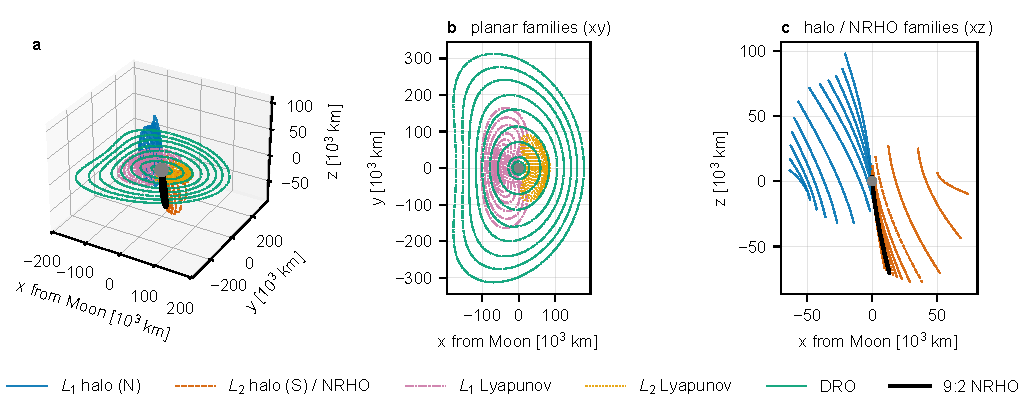
\includegraphics[width=\textwidth]{Fig1}
\caption{Earth--Moon CR3BP families used in this study (12 members of each family shown), in
Moon-centred coordinates: \textbf{a} three-dimensional view, \textbf{b} planar families in the
$xy$ plane, \textbf{c} halo and NRHO families in the $xz$ plane. The thick black curve is the 9:2
southern NRHO}\label{fig:families}
\end{figure}

\subsection{Sky geometry}\label{sec:geom}
To give the sky geometry real dates, the CR3BP trajectory is placed in the instantaneous
Earth--Moon frame of the actual Moon. The frame's $\hat x$ axis points from Earth to Moon, its
$\hat z$ axis lies along the Moon's orbital angular momentum, and distances scale with the constant
length unit. The Sun and Moon come from low-precision analytic series~\cite{montenbruck2000}, and
Earth rotation from Greenwich mean sidereal time. The Moon used in every geometric test is the
mapped CR3BP Moon, so the target--Moon geometry is exactly the CR3BP one. Truth, filters and
predictors share this mapping, so the setup is self-consistent; Section~\ref{sec:ephem} replaces it
with DE440~\cite{park2021}. The reference epoch is 2027-01-01 00:00\,UTC and the time grid spacing
is 10\,min.

\subsection{Sensors and visibility}\label{sec:sensors}
The network consists of Hanle (India), La Palma (Spain), Haleakala (USA) and Siding Spring
(Australia), in subsets of one site (India-1), three sites (Tri-3) and four sites (Tri-3+S). An
observation is possible only if all of the following hold: the Sun is below $-18^\circ$; the target
is above $20^\circ$ elevation; the line of sight misses the Moon; the target is outside Earth's and
the Moon's (cylindrical) shadows; the target is more than $\theta_{\mathrm{m}}$ from the Moon; and
the target is brighter than the effective limiting magnitude. The target is a Lambertian sphere of
radius 1\,m (2\,m diameter) and albedo 0.2, of magnitude 18.4 at zero phase angle at the Moon's
distance. The limiting magnitude is degraded by scattered moonlight following Krisciunas and
Schaefer~\cite{krisciunas1991}, and atmospheric extinction is applied. Dark-sky limiting magnitudes
of 19.5, 21.5 and 23.0 are assumed for 0.36, 1 and 2\,m apertures; the 0.36\,m value is anchored to
the CAPSTONE detection of Sechrest et al.~\cite{sechrest2024}. Measurements are topocentric right
ascension and declination with 1$''$ noise in each axis on the sky (isotropic, so the
right-ascension noise is $1''/\cos\delta$), every 10\,min per site when the target is visible.

\subsection{Estimators}\label{sec:estimators}
Four filters share one measurement model:
\begin{itemize}
\item an extended Kalman filter (EKF), with STM covariance propagation and Joseph-form updates;
\item an unscented Kalman filter (UKF) with 13 scaled sigma points ($\alpha=1$, $\beta=2$,
      $\kappa=0$);
\item a Gaussian-mixture UKF (GM-UKF). A component is split when its unscented prediction raises
      the differential entropy of its Gaussian fit by more than 0.02\,nats~\cite{demars2013}.
      Because the flow preserves volume, any entropy gain comes from nonlinear bending. The split
      is a moment-preserving three-way split along the direction of maximum stretching (the top
      right-singular vector of the statistically linearised flow multiplied by the Cholesky factor
      of the covariance). Pruning and Mahalanobis merging keep the mixture at no more than 40
      components;
\item a regularised bootstrap particle filter (PF) with progressive
      correction~\cite{oudjane2000,musso2001} and 3000 particles. It hands over to a UKF once its
      position uncertainty falls below 50\,km. Without the handover, the finite particle set
      impoverishes on long, dense arcs and its covariance drops below the Cram\'er--Rao bound.
\end{itemize}
The truth has no process noise. The filters carry a small white acceleration noise with power
spectral density $10^{-18}$\,km$^2$\,s$^{-3}$.

%% [Declaration of AI-assisted tools: to be written by the author here, in the Methods section, as required by JAS.]

%=====================================================================
\section{Custody Horizon: Definition and Computation}\label{sec:custody-def}

Let $(\hat{\vect x}_0, P_0)$ be the post-fit estimate at the last measurement before a gap. For
gap lengths $\Delta t \in [0.1, 30]$\,d (120 logarithmically spaced values), the uncertainty is
propagated three ways:
\begin{itemize}
\item \emph{linear}: $P(\Delta t) = \Phi P_0 \Phi^\top$, which is what an EKF predicts;
\item \emph{unscented} (UT): 13 sigma points, which is what a UKF predicts;
\item \emph{Monte Carlo} (MC): 300 samples of $\mathcal N(\hat{\vect x}_0, P_0)$ through the full
      dynamics, used as the reference.
\end{itemize}
The samples are projected onto the geocentric sky. For a search pattern of $N$ square fields of
view of side $\phi$, whose equal-area radius is $r_N = \phi\sqrt{N/\pi}$, the custody horizon is
\begin{equation}
\Tc(N) = \max\left\{\Delta t : \Pr\left[\angle(\hat{\vect u}_{\mathrm{target}}, \hat{\vect c}) \le r_N\right] \ge 0.99\right\},
\end{equation}
where $\hat{\vect c}$ is the centre of the search. Three variants use different centres or radii:
\begin{itemize}
\item \emph{ideal}: the circle is centred on the true (MC) mean direction;
\item \emph{actual}: the circle is centred on a method's own predicted direction;
\item \emph{claimed}: the time at which a method's \emph{own} 99\,\% region outgrows $r_N$.
\end{itemize}
The \emph{operator horizon} is the actual horizon of the UT prediction: the circle is centred where a
UKF would point the telescopes, so it uses no knowledge of the truth. It is the horizon reported in
Tables~\ref{tab:tc} and~\ref{tab:blackout}; the ideal horizon is the reference for the predictors of
Section~\ref{sec:predict}. A claimed horizon longer than the actual one is \emph{false custody}: the
predictor believes the target is still inside the pattern after it has left. Here $\phi = 1^\circ$ and
$N \in \{1, 10, 100\}$, giving search radii of 0.56$^\circ$, 1.78$^\circ$ and 5.64$^\circ$. Gaussian
\emph{containment} is the share of MC samples inside a method's 99\,\% sky ellipse (ideal value
99\,\%).

Because $\Tc$ is the \emph{first} gap at which the 99\,\% radius exceeds $r_N$, the gap grid must
resolve short excursions of the sky radius. On the NRHO the radius spikes at every perilune
passage (every 6.56\,d), when the along-track uncertainty is stretched as the object sweeps past
the Moon, and then shrinks again. The horizon is interpolated between grid points in log--log
coordinates. For 17
representative arcs, refining the grid to a uniform 0.02-d step changes $\Tc$ by a median of at
most 0.03\,d, by at most 0.15\,d for $N = 1$ and 10, and by at most 0.17\,d for $N = 100$.

The post-fit covariance at the gap start is the Cram\'er--Rao lower bound (CRLB) of the preceding
tracking arc of 1, 3 or 7\,days:
\begin{equation}
\mathcal I(t_0) = \Lambda_0 + \sum_k \Phi(t_k,t_0)^\top H_k^\top R^{-1} H_k \Phi(t_k,t_0),\qquad
P_0 = \Phi(t_e,t_0)\,\mathcal I^{-1}\,\Phi(t_e,t_0)^\top ,
\end{equation}
built from the actual visible measurements, with the gap starting at the arc's last measurement
$t_e$. Here $H_k$ is the Jacobian of right ascension and declination, $R$ the measurement noise
covariance ($\mathrm{diag}(\sigma^2/\cos^2\delta_k, \sigma^2)$ with $\sigma = 1''$, the same model as in the
simulated measurements and the filters), and $\Lambda_0$ a weak regularising prior ($10^5$\,km, 1\,km\,s$^{-1}$). An arc is
counted as observable when the resulting position bound is finite and below this prior.
Section~\ref{sec:filters} shows that the filters reach this bound in tracking. Two scenarios are
studied: arcs ending every 15\,days through the year (\emph{phase}), and arcs ending exactly when a
blackout of 2\,days or more begins (\emph{blackout}). Together they give 523 cases, of which 393 are
distinct arcs: a phase arc often ends exactly where a blackout begins, and then appears in both
scenarios. Statistics pooled over both scenarios use each distinct arc once.

A purely dynamical predictor is also tested: $\hat T_{\mathrm{FTLE}}$ is the first $\Delta t$ at
which the largest singular value of $\Phi$, $s_{\max}(\Phi(\Delta t)) = e^{\sigma_{\Delta t}\Delta t}$,
reaches $r_N/\theta_0$, where $\theta_0$ is the initial 99\,\% sky radius and $\sigma_{\Delta t}$ is
the FTLE~\cite{shadden2005}.

%=====================================================================
\section{Visibility: the Moon and the Lunar Phase Dominate}\label{sec:vis}

Seen from Earth, the four targets stay close to the Moon (Fig.~\ref{fig:sep}). The $L_1$ halo
stays within 3.9--6.1$^\circ$ and the $L_2$ Lyapunov orbit within 0--7.0$^\circ$. The NRHO ranges
over 0.5--10.0$^\circ$ (median 8.3$^\circ$), because it spends most of its time near apolune, and
the DRO over 0--13.9$^\circ$. All targets therefore stay within 14$^\circ$ of the Moon, and the
Moon-exclusion angle is the dominant sensor parameter (Table~\ref{tab:vis}). With a 10$^\circ$
exclusion, the $L_1$ and $L_2$ targets are never observable, whereas at 5$^\circ$ they are
observable 21--33\,\% of the year. At 5$^\circ$, doubling the aperture from 1 to 2\,m changes the
network's visible share by only 0.5--1.7 percentage points.

\begin{figure}[t]
\centering
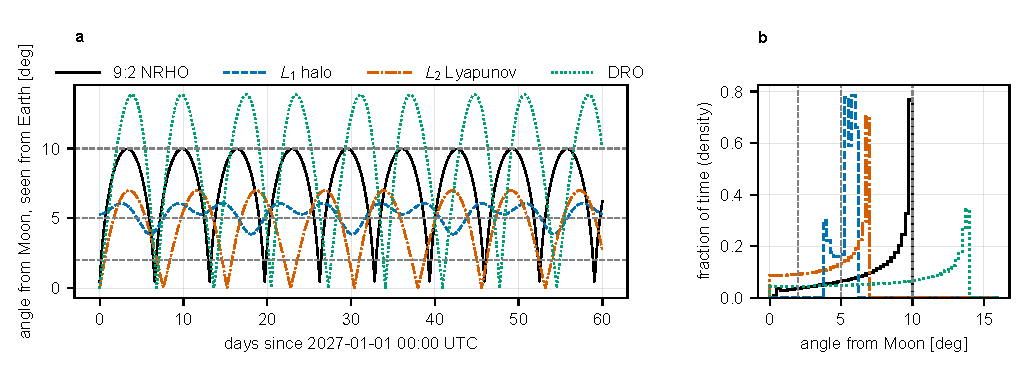
\includegraphics[width=\textwidth]{Fig2}
\caption{Geocentric angular separation between each target and the Moon: \textbf{a} 60-day time
series, \textbf{b} distribution over one year. Dashed lines mark the exclusion angles
studied}\label{fig:sep}
\end{figure}

\begin{table}[t]
\caption{One year of visibility (1\,m telescopes, Tri-3+S network): share of time observable and
longest observation gap, by Moon-exclusion angle $\theta_{\mathrm m}$}\label{tab:vis}
\begin{tabular*}{\textwidth}{@{\extracolsep\fill}lcccccc}
\toprule
 & \multicolumn{2}{c}{$\theta_{\mathrm m}=2^\circ$} & \multicolumn{2}{c}{$\theta_{\mathrm m}=5^\circ$} & \multicolumn{2}{c}{$\theta_{\mathrm m}=10^\circ$}\\
\cmidrule{2-3}\cmidrule{4-5}\cmidrule{6-7}
Orbit & Visible & Max gap & Visible & Max gap & Visible & Max gap\\
\midrule
9:2 NRHO       & 37.5\,\% & 12.8\,d & 31.4\,\% & 13.2\,d & 4.5\,\%  & 19.5\,d\\
$L_1$ halo     & 42.7\,\% & 11.2\,d & 32.6\,\% & 11.8\,d & 0\,\%    & ---\\
$L_2$ Lyapunov & 32.7\,\% & 13.5\,d & 20.6\,\% & 14.5\,d & 0\,\%    & ---\\
DRO            & 38.0\,\% & 11.8\,d & 32.5\,\% & 11.9\,d & 21.2\,\% & 16.5\,d\\
\botrule
\end{tabular*}
\end{table}

Visibility arrives in windows that run from roughly first quarter to last quarter
(Fig.~\ref{fig:timeline}): near new Moon the target lies close to the Sun on the sky and is up only
in daylight, and near full Moon the exclusion angle and scattered moonlight bite. Gap lengths fall
into three regimes (Fig.~\ref{fig:gaps}): handovers between sites (a few hours), diurnal gaps of
about 1\,d, which dominate for a single site, and multi-day lunar-phase blackouts. Adding sites or
aperture removes short gaps but not the lunar-phase blackout: at 5$^\circ$ exclusion, the longest
gap of the year is 8.5--15.7\,d for every network, 1--2\,m aperture and orbit.

\begin{figure}[t]
\centering
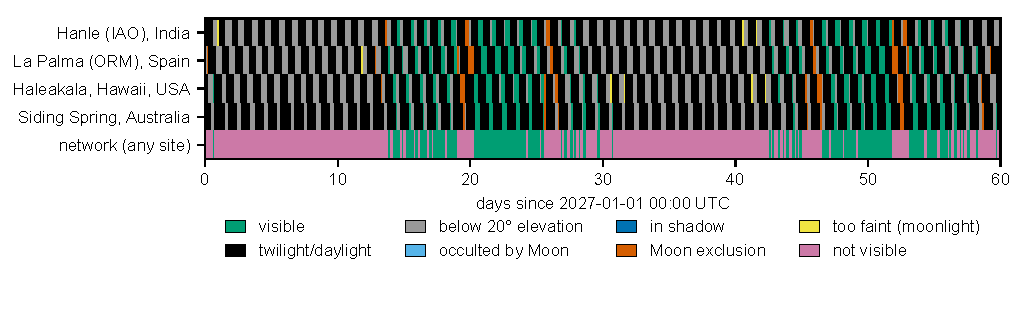
\includegraphics[width=\textwidth]{Fig3}
\caption{First blocking constraint per site for the 9:2 NRHO over 60 days (1\,m telescopes,
5$^\circ$ exclusion). The bottom row shows network availability}\label{fig:timeline}
\end{figure}

\begin{figure}[t]
\centering
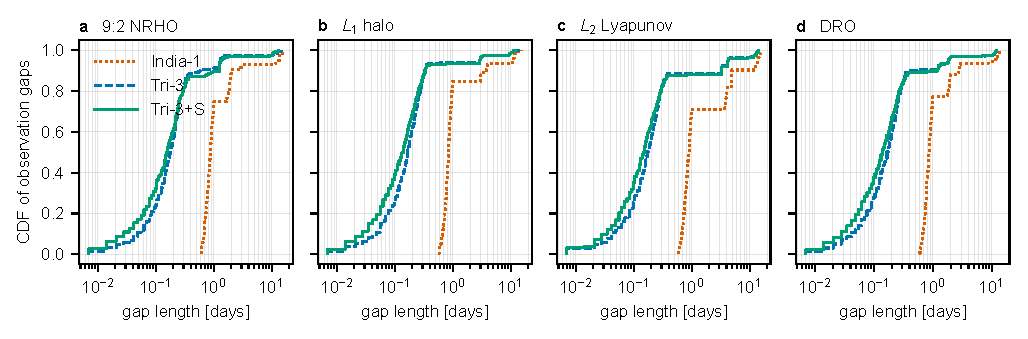
\includegraphics[width=\textwidth]{Fig4}
\caption{Cumulative distribution of observation gaps over one year (1\,m telescopes, 5$^\circ$
exclusion) for the three networks: \textbf{a} 9:2 NRHO, \textbf{b} $L_1$ halo, \textbf{c} $L_2$
Lyapunov, \textbf{d} DRO}\label{fig:gaps}
\end{figure}

%=====================================================================
\section{Observability and Filter Performance}\label{sec:filters}

\subsection{Cram\'er--Rao bounds}
Figure~\ref{fig:crlb} shows the bound, computed from the actual measurement schedule, for arcs
starting every 2\,days. At the end of 7-day arcs the median worst-direction position uncertainty
is 1.14\,km (NRHO), 1.83\,km ($L_1$ halo), 7.03\,km (DRO) and 17.8\,km ($L_2$ Lyapunov), and the
median velocity uncertainty is 6--108\,mm\,s$^{-1}$. Between 75\,\% and 84\,\% of 7-day arcs are
observable. For the DRO and the Lyapunov orbit, the weakest direction lies within 6.4--7.8$^\circ$
(median) of the line of sight, that is, it is essentially range. For the NRHO and the halo it lies
further from the line of sight (median 12.8--17.9$^\circ$), because the strongly curved dynamics
over a week also constrain range. Arcs that end inside a blackout show the uncertainty growth that
motivates the rest of the paper.

\begin{figure}[t]
\centering
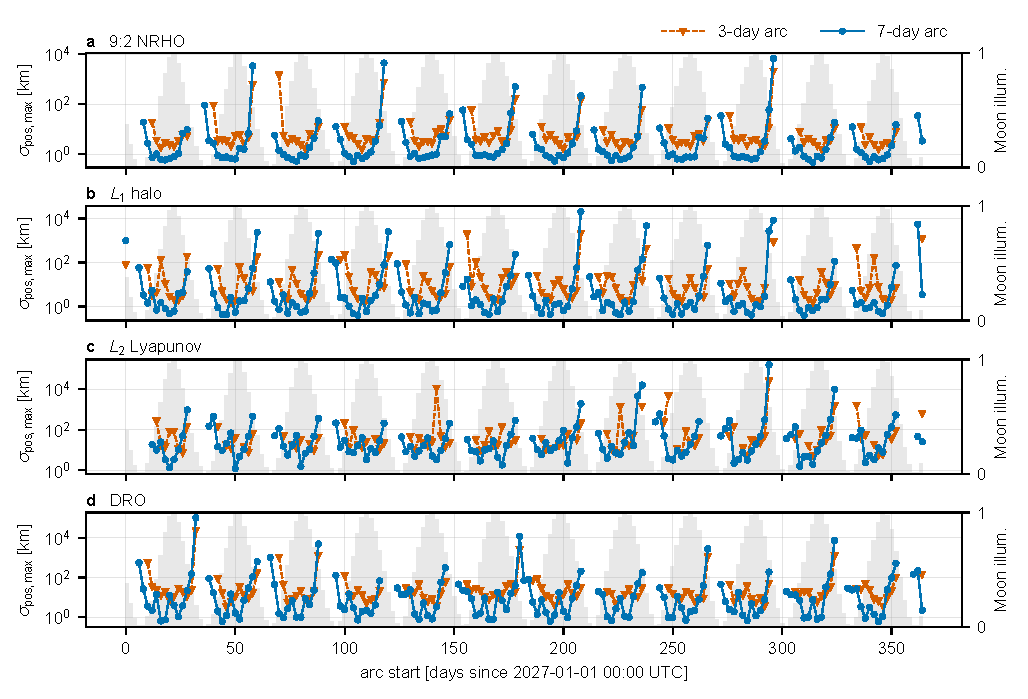
\includegraphics[width=\textwidth]{Fig5}
\caption{Cram\'er--Rao bound on the worst-direction position uncertainty at the end of 3-day and
7-day arcs, against the arc start date: \textbf{a} 9:2 NRHO, \textbf{b} $L_1$ halo, \textbf{c}
$L_2$ Lyapunov, \textbf{d} DRO. Grey shading shows lunar illumination; gaps are arcs that are not
observable}\label{fig:crlb}
\end{figure}

\subsection{Tracking}
When the filters are started at the first measurement of the arc from a 1000\,km /
10\,m\,s$^{-1}$ ($1\sigma$) prior, both the EKF and the UKF converge to the bound
(Table~\ref{tab:filters}, 20 Monte Carlo runs per orbit). The averaged NEES (ANEES, ideal value 6)
lies inside the 95\,\% band for 20 runs (4.58--7.61) for every orbit and both filters except the EKF
on the $L_2$ Lyapunov orbit, which is overconfident (9.25); the UKF on the same arc is consistent
(6.05).

\subsection{Reacquisition after a gap}
Reacquisition is tested on a separate 7-day arc per orbit that starts at the onset of the observation
gap closest to 3\,days, with the prior placed at the arc start. In the $L_1$ halo arc the first
measurement arrives 3.0\,d after the prior epoch. By then the 1000\,km prior has stretched into a
cloud whose 1--99\,\% extent is about $42\,000 \times 7600$\,km (Fig.~\ref{fig:cloud}). Over 100 runs,
only 37\,\% of EKF runs end consistent (95\,\% Wilson interval 28--47\,\%), with errors of up to
1793\,km while the filter claims about 36\,km. The UKF reaches 77\,\% (68--84\,\%), the PF with UKF
handover 88\,\% (80--93\,\%), and the GM-UKF 100\,\% (96--100\,\%) (Table~\ref{tab:filters},
Fig.~\ref{fig:reacq}). The GM-UKF splits into up to 27 components along the stretching direction,
averaging 3.0 components over the arc. All differences between the GM-UKF and the other three filters
are significant (Fisher exact test, $p \le 0.02$). On the other three orbits, with gaps of
1.9--3.2\,d, the UKF and the GM-UKF end consistent in 94--99\,\% of runs, the PF$\to$UKF in
91--95\,\% and the EKF in only 60--85\,\%. At the first measurement on the $L_1$ halo, the EKF's
99\,\% ellipsoid contains only 73\,\% of the particles, against 94\,\% for the UKF and 96\,\% for
the GM-UKF. After a 3-day gap the linear \emph{prediction} therefore already misses part of the
probability mass, and the measurement update, which linearises the angles across a $10^4$\,km cloud,
adds to the error.

\begin{table}[t]
\caption{Filter performance on 7-day arcs. Tracking: 20 runs, prior at the first measurement.
Reacquisition ($L_1$ halo, arc starting at a 3.0\,d observation gap): 100 runs, prior at the arc start; brackets give
95\,\% Wilson intervals; run times are wall-clock values on a laptop and machine dependent; the PF values vary slightly between platforms because resampling amplifies rounding differences. CRLB
and errors are position values in km (errors: RMS for tracking, median and maximum for
reacquisition). ``Consistent'' means the final NEES is below $\chi^2_{0.99}(6)$}\label{tab:filters}
\footnotesize
\begin{tabular}{@{}llcccc@{}}
\toprule
\multicolumn{6}{l}{\emph{Tracking}}\\
Orbit & CRLB & EKF error & EKF ANEES & UKF error & UKF ANEES\\
\midrule
9:2 NRHO       & 1.16  & 1.58  & 5.13 & 1.58  & 5.14\\
$L_1$ halo     & 1.83  & 1.94  & 5.71 & 1.97  & 5.36\\
$L_2$ Lyapunov & 17.88 & 9.60  & 9.25 & 9.50  & 6.05\\
DRO            & 7.16  & 6.05  & 5.13 & 6.15  & 5.15\\
\midrule
\multicolumn{6}{l}{\emph{Reacquisition, $L_1$ halo}}\\
Filter & Consistent & Median error & Max error & ANEES & Time [s]\\
\midrule
EKF         & 37\,\% (28--47)  & 68.0 & 1792.7 & $3.4\times10^3$ & 0.04\\
UKF         & 77\,\% (68--84)  & 31.0 & 251.5  & 64.0            & 0.06\\
GM-UKF      & 100\,\% (96--100) & 24.3 & 95.4  & 5.9             & 0.11\\
PF$\to$UKF  & 88\,\% (80--93)  & 27.6 & 1546.9 & $1.3\times10^3$ & 0.19\\
\botrule
\end{tabular}
\end{table}

\begin{figure}[t]
\centering
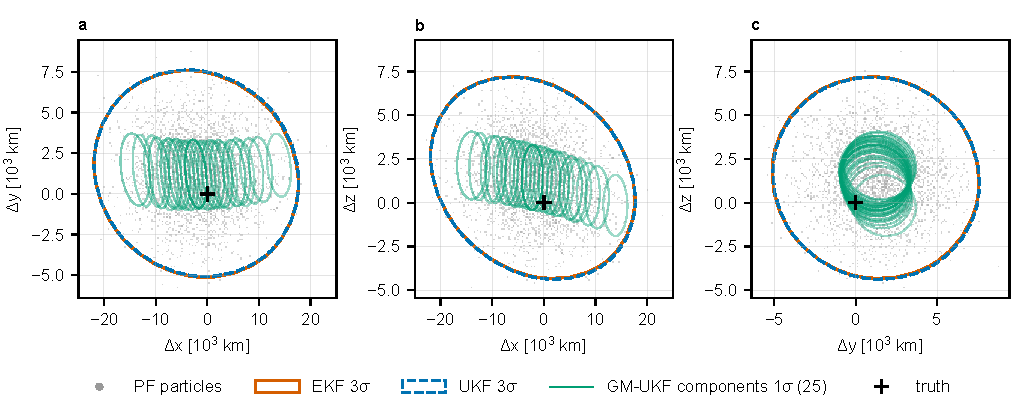
\includegraphics[width=\textwidth]{Fig6}
\caption{$L_1$ halo: predicted uncertainty at the first measurement after the 3.0-day initial gap
(run 0), relative to the truth, in the \textbf{a} $xy$, \textbf{b} $xz$ and \textbf{c} $yz$
synodic planes. Grey dots are PF particles; EKF and UKF $3\sigma$ ellipses and GM-UKF components
($1\sigma$) are shown}\label{fig:cloud}
\end{figure}

\begin{figure}[t]
\centering
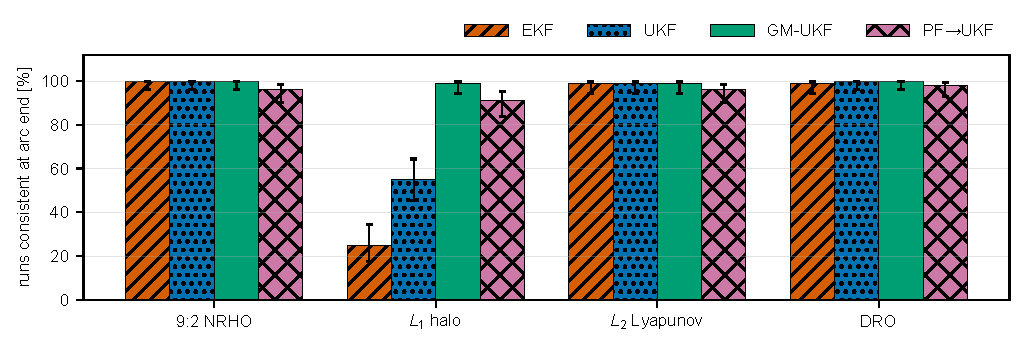
\includegraphics[width=\textwidth]{Fig7}
\caption{Share of reacquisition runs ending consistent, by filter and orbit (100 runs each); error
bars are 95\,\% Wilson intervals}\label{fig:reacq}
\end{figure}

%=====================================================================
\section{Custody Horizons}\label{sec:custody}

\subsection{Horizon maps}
Figure~\ref{fig:growth} shows how the true 99\,\% sky radius grows after 7-day arcs. The NRHO and
DRO stay below 0.01$^\circ$ for 30 days (median), reflecting their near-stability. The $L_1$ halo
and $L_2$ Lyapunov orbits grow roughly exponentially after about 5 days, and their median operator
horizons after 7-day arcs lie at 13.7--19.1\,d for one to 100 fields. Because the growth is so steep,
enlarging the search from 10 to 100 fields gains only 1.7--3.9 days (Table~\ref{tab:tc}). The
length of the tracking arc matters more: the $L_1$ halo's median horizon rises from 10.9 to
16.4\,d (10 fields) as the arc grows from 1 to 7 days. Over all arcs, the unstable orbits' median
horizons for a ten-field search lie at 10.9--17.3\,d.

The horizons in Tables~\ref{tab:tc} and~\ref{tab:blackout} are operator horizons: the search is
centred on the UT-predicted direction. Over all 393 distinct arcs they agree with the ideal horizons
(search centred on the true mean) to within 0.8\,d for $N \le 10$ and 1.5\,d for $N = 100$, with a
median ratio 1.00 for all three search sizes. When custody is lost, the UT-predicted centre is
therefore still much closer to the true mean than the search radius; custody ends because the
distribution outgrows the search, not because the search is centred in the wrong place.

\begin{figure}[t]
\centering
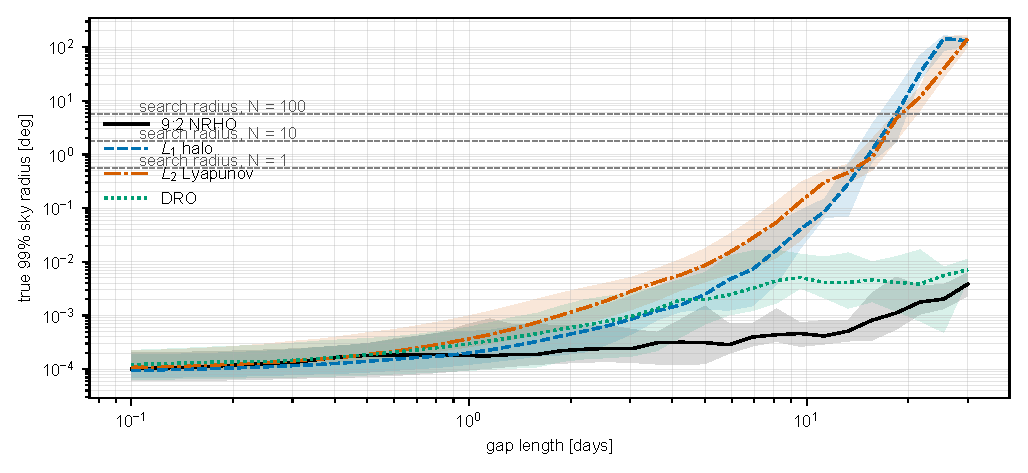
\includegraphics[width=\textwidth]{Fig8}
\caption{Growth of the true (Monte Carlo) 99\,\% sky radius after 7-day arcs: median and
10--90\,\% band over the year. Dashed grey lines are the search radii for 1, 10 and 100
one-degree fields}\label{fig:growth}
\end{figure}

\begin{table}[t]
\caption{Custody horizon $\Tc$ [days], median (10th--90th percentile) over arcs through the year
(phase scenario, operator horizon: search centred on the UT prediction); $\sigma_0$ is the median worst-direction position uncertainty at
the gap start. ``$>$30'' means beyond the 30-day grid}\label{tab:tc}
\begin{tabular*}{\textwidth}{@{\extracolsep\fill}llcccc}
\toprule
Orbit & Arc & $\sigma_0$ [km] & $N=1$ & $N=10$ & $N=100$\\
\midrule
9:2 NRHO       & 1\,d & 24.5 & $>$30 (5.3--$>$30) & $>$30 (18.4--$>$30) & $>$30\\
               & 3, 7\,d & 4.1, 0.9 & $>$30 & $>$30 & $>$30\\
$L_1$ halo     & 1\,d & 20.8 & 8.8 (5.5--9.9)   & 10.9 (7.3--12.2)  & 12.6 (9.5--13.7)\\
               & 3\,d & 5.1  & 11.6 (7.9--12.4) & 13.2 (10.0--14.1) & 14.9 (13.4--17.1)\\
               & 7\,d & 0.8  & 14.3 (13.0--15.3) & 16.4 (14.6--18.3) & 18.3 (16.3--19.9)\\
$L_2$ Lyapunov & 1\,d & 33.5 & 9.4 (7.6--10.9)  & 12.3 (9.7--15.4)  & 16.2 (12.8--18.0)\\
               & 3\,d & 16.2 & 10.3 (9.0--13.4) & 14.9 (11.2--16.4) & 18.0 (15.3--18.8)\\
               & 7\,d & 7.4  & 13.7 (11.6--15.7) & 17.3 (15.4--18.3) & 19.1 (18.3--21.1)\\
DRO            & 1\,d & 31.9 & $>$30 (7.8--$>$30) & $>$30 & $>$30\\
               & 3, 7\,d & 11.7, 1.4 & $>$30 & $>$30 & $>$30\\
\botrule
\end{tabular*}
\end{table}

\subsection{Blackouts}
The operational question is whether custody survives the blackouts that actually occur.
Figure~\ref{fig:blackout} and Table~\ref{tab:blackout} compare $\Tc$ with every blackout of 2 days
or more in the year. After 7-day arcs, every blackout is survived with a ten-field search. After
1-day arcs, 11--24\,\% of the blackouts are lost for the $L_1$ and $L_2$ targets, and 22\,\% for
the NRHO, whose blackouts last about 10.5\,d. The number of blackouts per orbit is small (9--34),
so the individual shares are uncertain by 10--30 percentage points (95\,\% Wilson intervals); the
ordering by arc length, however, holds for every orbit.

\begin{table}[t]
\caption{Blackouts ($\ge$2\,d) survived, that is, operator $\Tc \ge$ blackout length, by tracking-arc
length; $n$ is the number of blackouts with an observable preceding arc. The ideal horizon gives
the same shares except in one cell ($L_1$ halo, 1-day arcs, $N = 1$: 63\,\%)}\label{tab:blackout}
\begin{tabular*}{\textwidth}{@{\extracolsep\fill}llccccc}
\toprule
Orbit & Arc & $n$ & Median length & $N=1$ & $N=10$ & $N=100$\\
\midrule
9:2 NRHO       & 1\,d & 9  & 10.5\,d & 67\,\% & 78\,\%  & 78\,\%\\
               & 3\,d & 11 & 10.5\,d & 100\,\% & 100\,\% & 100\,\%\\
               & 7\,d & 11 & 10.5\,d & 100\,\% & 100\,\% & 100\,\%\\
$L_1$ halo     & 1\,d & 27 & 3.1\,d  & 67\,\% & 89\,\%  & 93\,\%\\
               & 3\,d & 27 & 3.1\,d  & 93\,\% & 96\,\%  & 96\,\%\\
               & 7\,d & 28 & 3.1\,d  & 100\,\% & 100\,\% & 100\,\%\\
$L_2$ Lyapunov & 1\,d & 33 & 4.1\,d  & 67\,\% & 76\,\%  & 94\,\%\\
               & 3\,d & 34 & 4.1\,d  & 79\,\% & 97\,\%  & 97\,\%\\
               & 7\,d & 34 & 4.1\,d  & 88\,\% & 100\,\% & 100\,\%\\
DRO            & 1\,d & 13 & 11.3\,d & 46\,\% & 85\,\%  & 85\,\%\\
               & 3\,d & 13 & 11.3\,d & 100\,\% & 100\,\% & 100\,\%\\
               & 7\,d & 13 & 11.3\,d & 100\,\% & 100\,\% & 100\,\%\\
\botrule
\end{tabular*}
\end{table}

\begin{figure}[t]
\centering
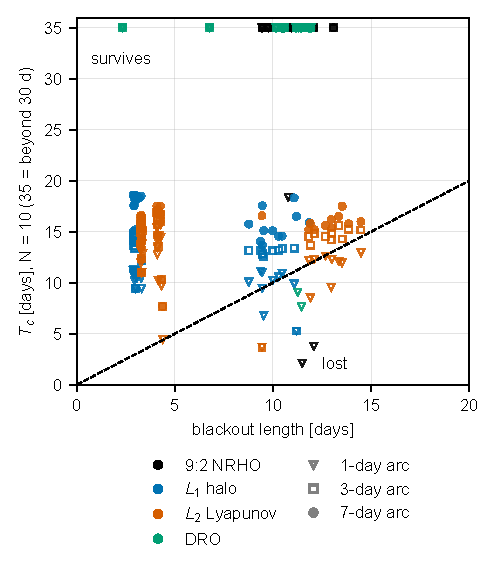
\includegraphics[width=0.5\textwidth]{Fig9}
\caption{Ideal custody horizon (ten fields; the operator horizon differs by at most 0.8\,d) against
blackout length. Points above the diagonal survive
the blackout; marker shape shows the tracking-arc length (open: 1 and 3 days, filled: 7 days)}\label{fig:blackout}
\end{figure}

%=====================================================================
\section{Predicting the Custody Horizon, and False Custody}\label{sec:predict}

Can $\Tc$ be predicted without Monte Carlo? Figure~\ref{fig:predict} compares the Monte Carlo
horizon with two cheap predictors, using the 250--270 distinct arcs (depending on the predictor and
$N$) whose horizons are finite and below 30\,d; $R^2$ is computed on the logarithm of the horizon.
The \emph{orbit-only} FTLE predictor fails, with log-$R^2$ between $-0.25$ and 0.04 for the three
search sizes. The \emph{covariance-based} predictors succeed: the UT predictor reaches
log-$R^2 = 0.96$, 1.00 and 0.93 for $N = 1$, 10 and 100 (bootstrap 95\,\% intervals 0.87--1.00,
0.99--1.00 and 0.85--0.98), and the linear predictor 0.92, 0.99 and 0.97. The FTLE measures stretching along the
flow's most unstable direction, but the post-fit covariance is highly anisotropic: angles-only data
constrain some directions far better than others, and only the uncertain directions that project
onto the sky matter for the search. Predicting custody requires the growth of the \emph{actual}
covariance, which the unscented transform supplies from 13 sigma points instead of hundreds of
samples.

\begin{figure}[t]
\centering
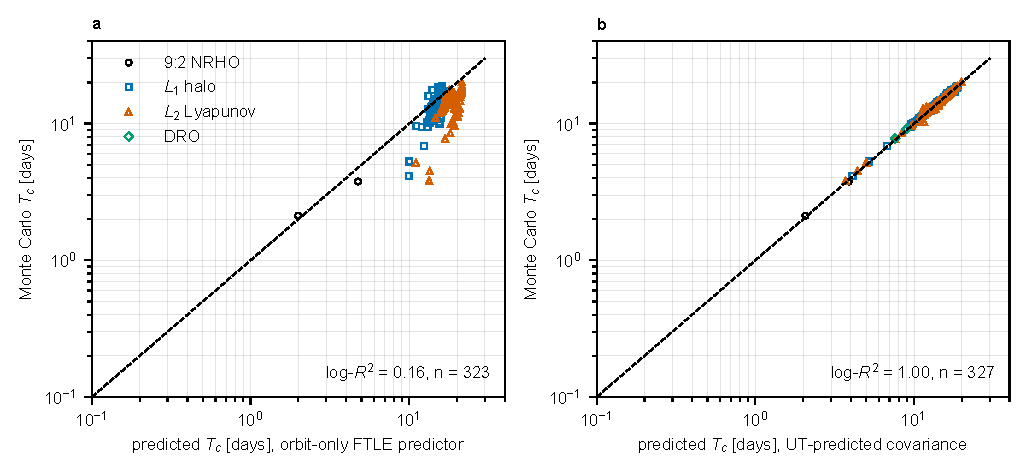
\includegraphics[width=\textwidth]{Fig10}
\caption{Monte Carlo custody horizon (ten fields) against \textbf{a} the orbit-only FTLE predictor
and \textbf{b} the horizon claimed by the UT-propagated covariance. The dashed line is equality}\label{fig:predict}
\end{figure}

Linear prediction is adequate for short gaps but breaks down on unstable orbits
(Fig.~\ref{fig:contain}). On the $L_1$ halo, the median linear containment first falls below 95\,\% at a gap
of 9.5\,d; on the $L_2$ Lyapunov orbit it does so only at 18.6\,d. After 14 days, the $L_1$ halo's linear 99\,\% sky ellipse
contains only 5.3\,\% of the true probability mass (median over all $L_1$ halo arcs), while the UT
ellipse contains 98\,\%. A search sized and shaped by the linear ellipse would therefore miss most of
the target's probability mass. The linear predicted centre, by contrast, generally stays close to the
true mean, so the linear failure lies mainly in the predicted spread rather than the predicted position. The UT-centred search gave false custody at $N = 10$ (a claimed horizon
more than 10\,\% longer than the actual one) in 2 of the 253 distinct arcs with a finite actual
horizon: an NRHO arc whose claim exceeds 30\,d while the UT-centred circle loses the target at
18.4\,d, and an $L_2$ Lyapunov arc claimed to 11.6\,d but lost at 10.2\,d. On the unstable orbits,
even the UT ellipse loses containment for long gaps: its median containment first falls below
95\,\% at 18.6--19.5 days and reaches minima of 65--72\,\%. The recovery near 30 days is an artefact of the small-angle projection once the
distribution covers tens of degrees, long after custody is lost.

\begin{figure}[t]
\centering
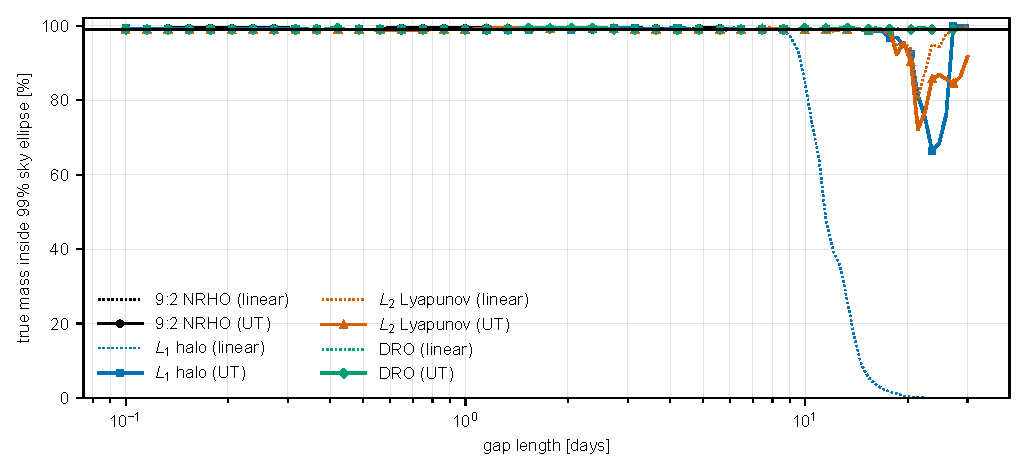
\includegraphics[width=\textwidth]{Fig11}
\caption{Share of the true probability mass inside the linear (dotted) and UT (solid, with
markers) 99\,\% sky ellipses, against gap length (median over 7-day arcs). The ideal value is
99\,\% (black line)}\label{fig:contain}
\end{figure}

%=====================================================================
\section{Ephemeris Cross-Check}\label{sec:ephem}

The CR3BP results are checked in an Earth-centred ephemeris model with DE440 Sun and Moon point
masses~\cite{park2021} and cannonball solar radiation pressure (area-to-mass ratio
0.01\,m$^2$\,kg$^{-1}$, $C_r = 1.3$, cylindrical Earth shadow). Each orbit is first transitioned to
its ephemeris counterpart by multiple shooting over 45-day windows. Patch points are placed every
0.1 periods and corrected by Levenberg--Marquardt followed by minimum-norm Newton iterations, with
STMs from the gravity-gradient variational equations. The $L_1$ halo, $L_2$ Lyapunov and DRO
counterparts are continuous to better than 0.4\,m and stay within 3500--5200\,km (median) of their
CR3BP shapes. The NRHO counterpart retains a continuity residual of 50--124\,km (median to
maximum over windows), because the corrector stalls in the ill-conditioned perilune segments; this
is a limitation of the present corrector. For 60 custody cases (58 distinct arcs; blackout and
phase scenarios, 1- and 7-day arcs), the CRLB covariance is mapped to inertial coordinates and propagated in the
ephemeris model.

The conclusions carry over (Figs.~\ref{fig:ephem} and~\ref{fig:ephemgrowth},
Table~\ref{tab:ephem}). The median ratio of ephemeris to CR3BP horizon is 0.93--1.00, and the
growth curves overlap. In 5 of the 58 distinct arcs, local differences in the ephemeris dynamics
shift $\Tc$ by more than 3 days or across the 30-day limit. Blackout survival is
unchanged except for one single-case difference in a four-case group ($L_1$ halo, 1-day arcs). The UT
predictor again reaches log-$R^2 = 1.00$ for $N = 10$, but only 0.80 for $N = 1$ (41 finite cases,
bootstrap interval 0.37--1.00) and 0.83 for $N = 100$ (30 finite cases, bootstrap interval 0.58--0.99).
With so few finite cases these two values are uncertain; at a search radius of 5.6$^\circ$, moreover,
the distribution is too curved for any single Gaussian. Linear false custody
persists, and on the $L_2$ Lyapunov orbit it becomes \emph{worse}. At 14 days the linear ellipse
holds 12.0\,\% of the mass for the $L_1$ halo (9.9\,\% for the same arcs in the CR3BP) and 79.9\,\%
for the $L_2$ Lyapunov orbit (98.7\,\% in the CR3BP), while the UT ellipse holds 98--99\,\%.

\begin{table}[t]
\caption{Ephemeris (DE440 + solar radiation pressure) versus CR3BP: median custody horizon (ten
fields) and median ratio, by tracking-arc length}\label{tab:ephem}
\begin{tabular*}{\textwidth}{@{\extracolsep\fill}llcccc}
\toprule
Orbit & Arc & $n$ & CR3BP $\Tc$ & Ephemeris $\Tc$ & Ratio\\
\midrule
9:2 NRHO       & 1\,d & 8  & $>$30\,d & 28.3\,d  & 0.98\\
               & 7\,d & 7  & $>$30\,d & $>$30\,d & ---\\
$L_1$ halo     & 1\,d & 4  & 8.4\,d   & 7.8\,d   & 0.93\\
               & 7\,d & 11 & 15.9\,d  & 15.8\,d  & 1.00\\
$L_2$ Lyapunov & 1\,d & 5  & 11.9\,d  & 11.3\,d  & 0.95\\
               & 7\,d & 10 & 15.8\,d  & 16.4\,d  & 1.00\\
DRO            & 1\,d & 6  & $>$30\,d & $>$30\,d & 1.00\\
               & 7\,d & 9  & $>$30\,d & $>$30\,d & ---\\
\botrule
\end{tabular*}
\end{table}

\begin{figure}[t]
\centering
\begin{minipage}[t]{0.48\textwidth}\centering
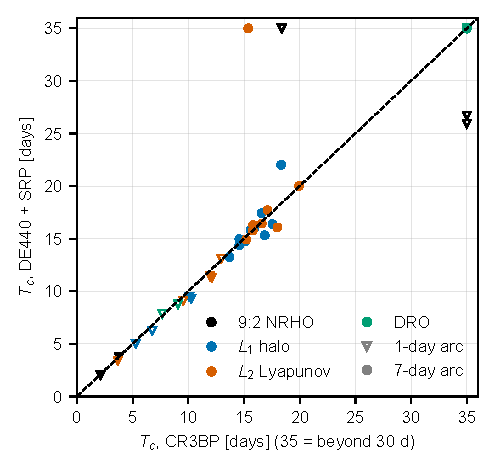
\includegraphics[width=\textwidth]{Fig12}
\caption{Custody horizon in the CR3BP and in the ephemeris model (ten fields); open markers: 1-day
arcs, filled: 7-day arcs}\label{fig:ephem}
\end{minipage}\hfill
\begin{minipage}[t]{0.48\textwidth}\centering
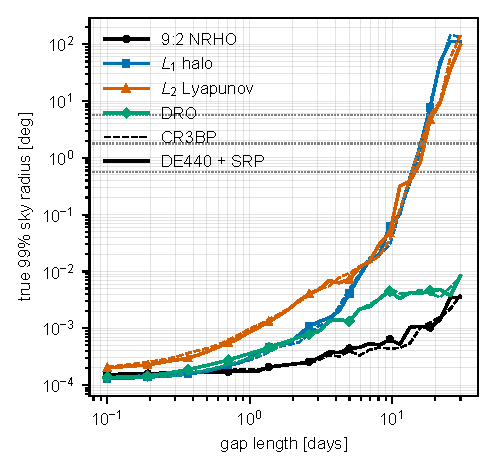
\includegraphics[width=\textwidth]{Fig13}
\caption{Median sky-radius growth after 7-day arcs: CR3BP (dashed) and ephemeris (solid). Dotted
grey lines are the search radii}\label{fig:ephemgrowth}
\end{minipage}
\end{figure}

%=====================================================================
\section{Horizon Across Orbit Families}\label{sec:families}

The four representative orbits do not show whether the horizon is a property of the particular orbit or
of its family's dynamics. The custody computation of Section~\ref{sec:custody-def} is therefore
repeated for members of all five families of Section~\ref{sec:dyn}. Up to eight members are taken
evenly along each family among those that stay more than 200\,km above the lunar surface. Members
observable for less than 1\,\% of the year or without an observable arc are dropped, and 30 members
remain (seven $L_1$ halo, seven $L_2$ halo and NRHO, six $L_1$ Lyapunov, five $L_2$ Lyapunov and five
DRO members). Each member starts at a random orbital phase at the epoch. Tracking arcs of 3 and
7\,days end at the last visible measurement before each of eight dates 45\,days apart, observed by the
reference sensors (1\,m telescopes, Tri-3+S network, 5$^\circ$ exclusion), which gives 413 cases. The
stability index of a member is $\nu = \max |\lambda + 1/\lambda|/2$ over the eigenvalues $\lambda$ of
its monodromy matrix; $\nu = 1$ means linearly stable.

\subsection{Stability index}
Figure~\ref{fig:stability} shows the operator horizon against $\nu$. After 7-day arcs, all 15 members
with $\nu < 3$ (every DRO, six of the seven $L_2$ halo and NRHO members and four $L_1$ halo members)
keep custody beyond 30\,d (member median). After 3-day arcs all but two of them do; the exceptions are
two $L_1$ halo members with $\nu = 2.4$ and 2.9, lost at 29.1 and 26.9\,d. Above $\nu = 10$ the horizon falls as $\nu$ grows:
after 7-day arcs the finite member medians span 12.9--25.2\,d, and two $L_1$ Lyapunov members
($\nu = 71$ and 113) stay beyond 30\,d. For the 15 members with $\nu > 10$, the Spearman rank
correlation between the member median horizon and $\log\nu$ is $\rho = -0.92$ (3-day arcs) and
$-0.91$ (7-day arcs), both with $p < 10^{-5}$; horizons beyond 30\,d enter as ties at 30\,d.
Including the nearly stable members (all 25 members with $\nu > 1.01$; the DROs have $\nu = 1.00$)
gives $-0.97$ and $-0.91$.

Within families, the correlation is strong for the $L_1$ halo and both Lyapunov families ($\rho$
between $-0.91$ and $-1.00$ for both arc lengths, with five to seven members each). The $L_2$ halo
family is the exception, with $\rho = -0.61$ ($p = 0.14$) for both arc lengths. Six of its seven
members are nearly stable ($\nu \le 1.7$) and keep custody beyond 30\,d, so only one member
($\nu = 75$) carries ranking information, and this family on its own neither supports nor contradicts
the trend.

The stability index therefore separates orbits that keep custody for a month from orbits that do not,
and it orders the unstable ones. It does not predict individual cases: at a given $\nu$ the horizon
varies by several days from arc to arc (vertical lines in Fig.~\ref{fig:stability}). This agrees with
Section~\ref{sec:predict}. The index ranks members by their median horizon over a year, whereas the
horizon after a particular arc is set by that arc's post-fit covariance, which no orbit-only quantity
such as the FTLE can supply.

\begin{figure}[t]
\centering
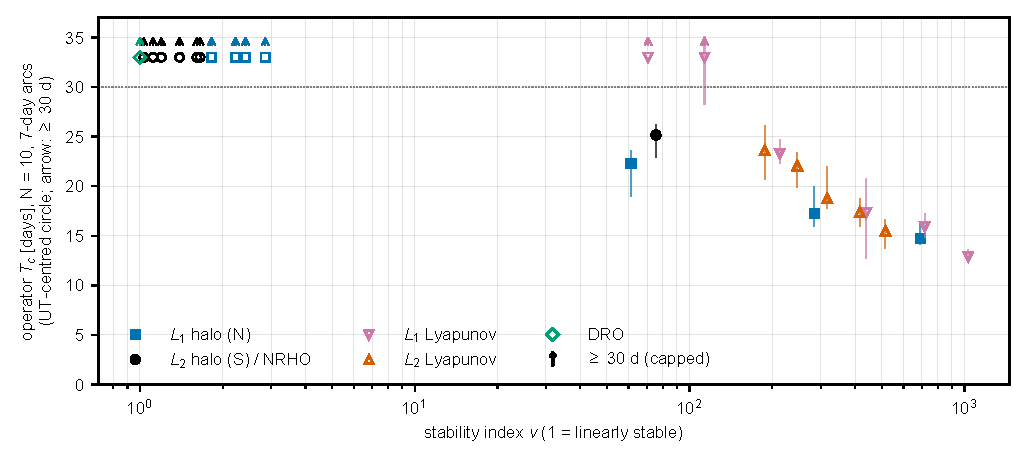
\includegraphics[width=\textwidth]{Fig14}
\caption{Operator custody horizon (UT-centred circle, ten fields, 7-day arcs) against the stability
index $\nu$ for 30 members of five families: median over arcs (markers) and 10--90\,\% range over
arcs (vertical lines). Members whose median exceeds 30\,d are drawn above the dotted line with an
arrow. Open markers: Lyapunov families and members beyond 30\,d}\label{fig:stability}
\end{figure}

\subsection{Operator and strip searches}
Over all 413 cases, the operator horizon differs from the ideal one by at most 0.17\,d for $N = 1$,
0.38\,d for $N = 10$ and 1.18\,d for $N = 100$, and the median ratio of the two is 1.00 for all three
search sizes (Fig.~\ref{fig:opideal}a). The result of Section~\ref{sec:custody} therefore holds across
the families: centring the search on the unscented prediction costs no custody time.

An operator can also exploit the elongation of the predicted uncertainty by laying out the $N$ fields
as a strip along the major axis of the UT-predicted sky ellipse, with the aspect ratio of the ellipse,
at most 10$^\circ$ long, and taking the worst of orientation errors of $\pm2^\circ$. Relative to the
ideal circle, the median horizon of this strip is 0.97, 1.08 and 0.98 for $N = 1$, 10 and 100
(Fig.~\ref{fig:opideal}b). At $N = 10$, the strip gains more than 3\,d in 54 of the 206 cases with a
finite ideal horizon, 49 of them on the Lyapunov families. These are the cases whose true distribution
is thinnest across the strip: where the circle loses custody, the 99\,\% cross-track half-width of the
distribution is 0.6$''$ (median), against 1.5$''$ for the other cases. Such thin distributions follow
from a Cram\'er--Rao covariance without measurement biases, timing errors or force-model errors. The
strip gain is therefore reported as a possible improvement that remains to be confirmed with a more
realistic covariance, not as a result.

\begin{figure}[t]
\centering
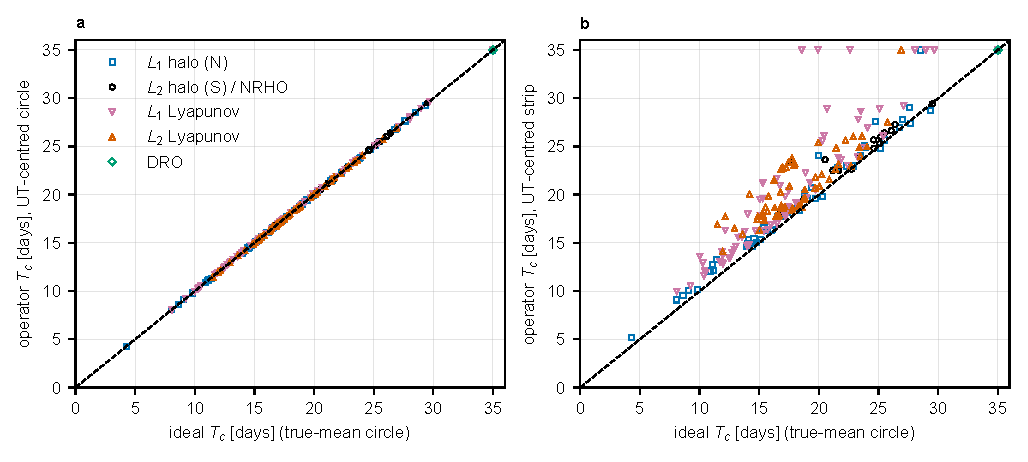
\includegraphics[width=\textwidth]{Fig15}
\caption{Operator against ideal custody horizon (ten fields) for the 413 family-sweep cases:
\textbf{a} circle centred on the UT prediction, \textbf{b} strip along the UT-predicted sky ellipse.
Horizons beyond 30\,d are plotted at 35\,d; the dashed line is equality}\label{fig:opideal}
\end{figure}

%=====================================================================
\section{Robustness to Unmodelled Errors}\label{sec:consider}

The horizons so far start from the Cram\'er--Rao bound, which assumes that white measurement noise is
the only error. Real astrometry also has errors that do not average down with the number of
measurements. They are added here as consider parameters~\cite{tapley2004}: quantities that the
estimator does not solve for, but whose uncertainty enters the error of its estimate. The measurements
become $\vect z_k = h(\vect x_k) + \vect b_s + \vect b_c + \vect v_k$, with a constant angle bias
$\vect b_s$ per site and sky axis, a common bias $\vect b_c$ shared by all sites (for example catalogue
zonal errors or a common reduction pipeline), and a constant clock offset per site. The dynamics get an
error in the area-to-mass ratio $A/m$ of a cannonball solar radiation pressure model ($C_r = 1.3$),
which acts during the arc and keeps acting during the gap. Two cases are distinguished: the operator
models solar radiation pressure but $A/m$ is uncertain by 30\,\% (for $A/m$ from 0.005 to
0.05\,m$^2$\,kg$^{-1}$), or the operator does not model it at all, so that the truth carries the full
$A/m$. With $S$ the sensitivity of the least-squares estimate to the consider parameters, mapped to the
arc end, and $C$ their covariance, the arc-end covariance becomes
$P = P_{\mathrm{CRLB}} + S C S^\top$. This covariance, together with the solar-pressure error during the
gap, defines the Monte Carlo truth; the operator still plans with the Cram\'er--Rao covariance and the
unperturbed CR3BP, as in Section~\ref{sec:custody}. The nominal case combines a 0.1$''$ bias per site, a
1\,ms clock offset and $A/m = 0.01 \pm 30\,\%$; the conservative case combines 0.5$''$ per site, a
0.1$''$ common bias, 10\,ms and $A/m = 0.05 \pm 30\,\%$. Both are also run with 0.3$''$ instead of 1$''$
white noise. The study uses the phase arcs every 30\,days (126 arcs of 1, 3 and 7\,days); without the
additional errors it reproduces the horizons of Section~\ref{sec:custody} exactly.

The horizons hold (Fig.~\ref{fig:consider}). For a ten-field search and the 67 arcs whose reference
horizon is below 30\,d, the nominal errors shorten the operator horizon by a median of 1\,\% (ratio
0.99, 10th percentile 0.96). A per-site bias costs little up to 0.2$''$ (ratio 0.99) and 5\,\% at 0.5$''$
(ratio 0.95, with 5 arcs losing more than 20\,\%). A common bias matters less than independent site
biases, and clock offsets have no effect: the targets move across the sky at a median of
0.4$''$\,s$^{-1}$ and, in 95\,\% of the measurements, at less than 0.7$''$\,s$^{-1}$, so 10\,ms shifts
them by a few milliarcseconds. With solar radiation pressure modelled, the median ratio stays
at 0.98--1.00 up to $A/m = 0.05$\,m$^2$\,kg$^{-1}$, although the 10th percentile falls to 0.82. Not
modelling solar radiation pressure at all is the largest single effect: at $A/m = 0.05$\,m$^2$\,kg$^{-1}$
the median ratio is 0.94 and 8 arcs lose more than 20\,\%. It is also the only error that moves the
centre of the search: the truth drifts away from the prediction, so the operator horizon falls while the
ideal horizon hardly changes (ratio 0.99). The conservative case gives a median ratio of 0.93 (10th
percentile 0.71, 13 arcs losing more than 20\,\%). The near-stable orbits are barely affected: at most
2 of the 28 NRHO arcs fall below 30\,d, and no DRO arc does.

Systematic errors matter more when the white noise is smaller. With 0.3$''$ noise the horizons
themselves are longer, by a median of 1.8\,d, but the nominal errors then cost 4\,\% (ratio 0.96) and the
conservative errors 19\,\% (ratio 0.81, with 46\,\% of the arcs losing more than 20\,\%), because the
biases dominate the post-fit covariance.

What does not hold is the Cram\'er--Rao claim. An operator who sizes the search from the Cram\'er--Rao
covariance claims a horizon more than 10\,\% longer than the actual one in 1.5\,\% of the arcs without
the additional errors, in 9\,\% under the nominal errors, in 34\,\% with 0.5$''$ site biases, and in
82\,\% for the conservative errors with 0.3$''$ noise. The search should therefore be sized from a
covariance inflated for these errors, such as the consider covariance used here.

\begin{figure}[t]
\centering
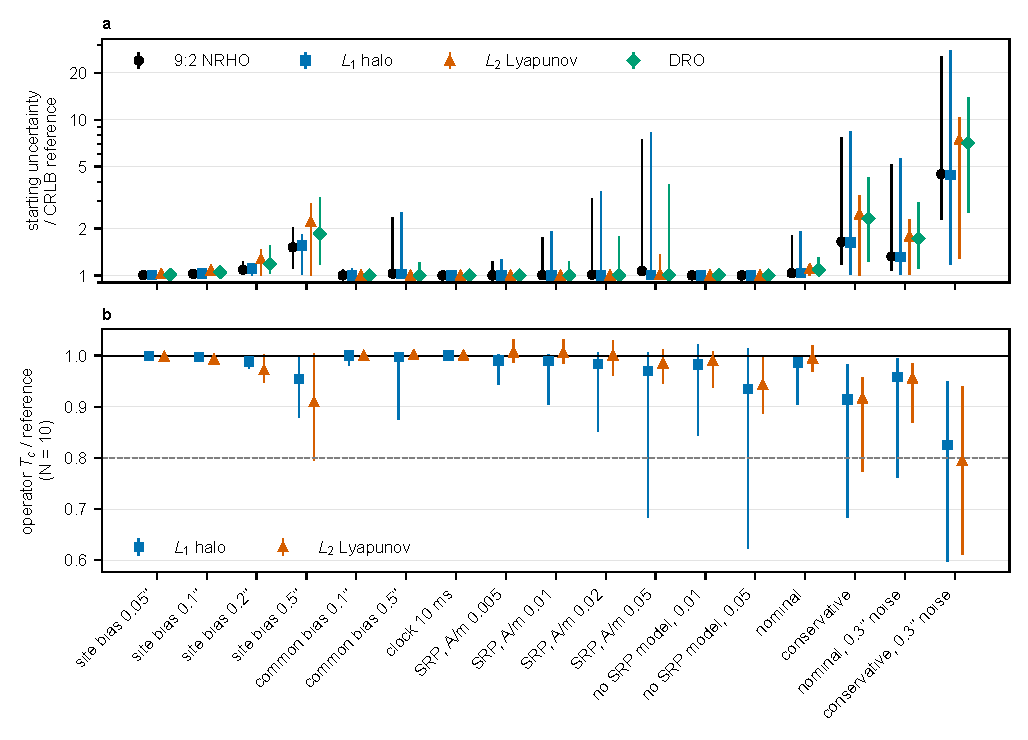
\includegraphics[width=\textwidth]{Fig16}
\caption{Effect of unmodelled errors on custody: \textbf{a} starting uncertainty relative to the
Cram\'er--Rao reference (largest $1\sigma$ position axis), \textbf{b} operator horizon (ten fields)
relative to the reference for the arcs whose reference horizon is below 30\,d. Markers are medians and
lines 10--90\,\% ranges. Configurations: per-site bias, common bias, clock offset, solar radiation
pressure modelled with $A/m$ uncertain by 30\,\%, solar radiation pressure not modelled, and the
nominal and conservative combinations, the last two also with 0.3$''$ white noise (reference: the
0.3$''$ Cram\'er--Rao bound). An unmodelled force shifts the mean rather than widening the covariance,
so its value in \textbf{a} is 1. The dashed line marks a 20\,\% loss}\label{fig:consider}
\end{figure}

%=====================================================================
\section{Discussion}\label{sec:discussion}

\subsection{Operational implications}
Six rules follow from the results.
\begin{enumerate}
\item Sensor design for cislunar tracking from the ground should minimise the usable
      Moon-exclusion angle (baffling, scattered-light rejection) before increasing aperture.
\item The monthly lunar-phase blackout cannot be closed by adding ground sites. Custody through it
      depends on the post-fit covariance, so tasking should concentrate at least 3 and preferably
      7\,days of tracking before each predicted blackout.
\item Search planning after a gap should use unscented (or Gaussian-mixture) prediction; in the CR3BP,
      linear prediction on the $L_1$ halo is safe only for gaps shorter than about 10\,days, and in
      the ephemeris model it also fails on the $L_2$ Lyapunov orbit by 14\,days (Section~\ref{sec:ephem}).
\item Reacquisition after a long gap should use a Gaussian-mixture filter, which costs about twice
      as much as a UKF; it was the only filter to end consistent in at least 99\,\% of the $L_1$ halo reacquisition runs.
\item On the NRHO, a narrow (single-field) search should be scheduled away from perilune, where the
      sky-plane uncertainty briefly swells before shrinking again (Section~\ref{sec:custody-def}).
\item The search size should come from a covariance inflated for site biases and solar-pressure
      errors, not from the Cram\'er--Rao bound: the horizons are robust to these errors, but
      Cram\'er--Rao claims of custody become false in a third of the arcs once site biases reach
      0.5$''$ (Section~\ref{sec:consider}). Solar radiation pressure should be modelled.
\end{enumerate}
Because the operator horizon matches the ideal one, these horizons are achievable by an operator who
centres the search on a UKF prediction. The stability index gives a first screening of a catalogue: in
this study, members with $\nu < 3$ kept custody beyond 30\,days after 7-day arcs, while members with
$\nu > 10$ needed re-observation within two to four weeks (Section~\ref{sec:families}). For the
individual arc, the UT predictor tracks the Monte Carlo horizon closely for $N \le 10$ and could be
evaluated inside a tasking scheduler for every catalogued object at negligible cost.

\subsection{Limitations}
\begin{itemize}
\item This is a simulation study; no real observations are processed.
\item The post-fit covariance is the Cram\'er--Rao bound, which the filters reach in tracking but
      not always immediately after a gap. Section~\ref{sec:consider} adds site biases, clock offsets
      and solar-pressure errors for 126 arcs of the four representative orbits; the family sweep and
      the strip gains of Section~\ref{sec:families}, which rest on very thin distributions, were not
      re-tested with them.
\item Sensor parameters (limiting magnitudes, extinction, dark-sky brightness) are nominal. The
      moonlight model of Krisciunas and Schaefer~\cite{krisciunas1991} is extrapolated below
      10$^\circ$ from the Moon, and the exclusion angle stands in for instrument-specific scattered
      light.
\item Targets are passive, non-manoeuvring spheres of 2\,m diameter, and data association and
      clutter are not modelled.
\item Each 99\,\% quantile is estimated from 300 samples. Re-running 17 representative arcs with
      2000 samples changes $\Tc$ by a median of 0.08--0.13\,d (1--2\,\%) and by at most 0.7\,d for
      $N = 10$ and 100. At $N = 1$, one NRHO arc whose 99\,\% radius only just reaches the search
      radius during a perilune passage moves from 5.3 to 17.6\,d.
\item The NRHO ephemeris counterpart is not fully continuous.
\item The CR3BP study places orbits in the real Earth--Moon direction with analytic ephemerides, and
      the DE440 check covers 60 of the 523 cases.
\end{itemize}

\subsection{Future work}
The main next step is validation with real observations, by proposing observing requests at Indian
facilities (the 2\,m Himalayan Chandra Telescope at Hanle, the telescopes of the Aryabhatta Research
Institute of Observational Sciences at Devasthal, and the 0.7\,m GROWTH-India robotic telescope) for
targets and nights selected from the custody maps. Other extensions are custody-aware sensor
tasking that uses the UT-predicted $\Tc$, mixed ground and space-based networks, and manoeuvre
detection.

%=====================================================================
\section{Conclusions}\label{sec:conclusions}

The custody horizon was defined for ground-based, angles-only tracking of cislunar periodic orbits
and mapped over a year of physically generated observations, for a search centred on the operator's
own unscented prediction. This operator horizon equals that of an idealised search centred on the true
mean (median ratio 1.00), so the horizons reported here can be achieved in practice. The targets
studied stay within 14$^\circ$ of the Moon, so the exclusion angle and the lunar phase control
visibility, and monthly blackouts of up to two weeks are unavoidable from the ground. The near-stable
9:2 NRHO and DRO keep custody for more than 30 days after three or more days of tracking. The unstable
$L_1$ halo and $L_2$ Lyapunov orbits keep it for 11--17\,days (median, ten fields), with the
tracking-arc length before a gap as the controlling factor. Across 30 members of five orbit families,
nearly stable members keep custody beyond 30 days and, above a stability index of 10, the horizon falls
with the index (Spearman $\rho = -0.92$ and $-0.91$ for 3- and 7-day arcs). The horizon after an
individual arc is predicted closely by the unscented transform of the post-fit covariance, but not by
the orbit's FTLE alone, and linear prediction gives false custody on unstable orbits after long gaps.
Realistic site biases, clock offsets and solar-pressure errors shorten the horizons by about 1\,\% at
nominal levels and by 7\,\% (median) in a conservative case, but make custody claims based on the
Cram\'er--Rao covariance overconfident, so the search should be sized from an inflated covariance.
After a 3-day gap on the $L_1$ halo, a Gaussian-mixture UKF reacquired in all 100 runs, against
37\,\% for the EKF and 77\,\% for the UKF. The main conclusions are reproduced, for 60 of the 523 cases,
in a DE440 ephemeris model with solar radiation pressure.

%=====================================================================
\bmhead{Acknowledgements}
%% Acknowledgements (supervisor, colleagues, computing). JAS places them on the title page.
None.

\section*{Declarations}

\bmhead{Funding}
%% CHECK: state any fellowship or grant that supported the author.
The author did not receive support from any organization for the submitted work.

\bmhead{Competing interests}
The author has no relevant financial or non-financial interests to disclose.

\bmhead{Data and code availability}
%% CHECK: make the repository public and insert the Zenodo DOI before submission.
The code (CR3BP and ephemeris dynamics, sensor model, estimators, custody analysis and unit tests),
the scripts that regenerate every figure and table, the generated data, and a script that checks
every number in this paper against those data are available in the \texttt{cislunar-custody}
repository (\url{https://github.com/Bishwaswarup/cislunar-custody}), archived at Zenodo
(\url{https://doi.org/10.5281/zenodo.XXXXXXX}).

\bmhead{Author contributions}
B.N. conceived the study, developed the software, performed the analysis and wrote the manuscript.

\bmhead{Ethics approval and consent to participate}
Not applicable.

\begin{appendices}
\section{Reference Parameters}\label{app:params}
\begin{table}[h]
\caption{Reference parameters of the simulations}\label{tab:params}
\begin{tabular*}{\textwidth}{@{\extracolsep\fill}lp{0.72\textwidth}}
\toprule
Quantity & Value\\
\midrule
CR3BP & $\mu = 0.0121505842$, length unit 384\,400\,km, time unit 4.3425\,d\\
Epoch, grid & 2027-01-01 00:00 UTC, 10\,min, one year\\
Sites & Hanle (32.78$^\circ$N, 78.96$^\circ$E, 4.5\,km); La Palma (28.76$^\circ$N, 17.88$^\circ$W, 2.4\,km); Haleakala (20.71$^\circ$N, 156.26$^\circ$W, 3.05\,km); Siding Spring (31.27$^\circ$S, 149.06$^\circ$E, 1.16\,km)\\
Constraints & Sun $< -18^\circ$; elevation $> 20^\circ$; exclusion 2/5/10$^\circ$ (reference 5$^\circ$); no occultation; sunlit\\
Telescopes & limiting magnitude 19.5 / 21.5 / 23.0 for 0.36 / 1 / 2\,m (reference 1\,m)\\
Target & Lambertian sphere, radius 1\,m, albedo 0.2\\
Measurements & topocentric right ascension and declination, $\sigma = 1''$, every 10\,min per site when visible\\
Filters & prior 1000\,km / 10\,m\,s$^{-1}$; process-noise PSD $10^{-18}$\,km$^2$\,s$^{-3}$; UKF $\alpha=1$, $\beta=2$, $\kappa=0$; GM split threshold 0.02\,nats, $\le$40 components; PF 3000 particles, handover at 50\,km; tracking 20 runs, reacquisition 100 runs\\
CRLB & weak prior $10^5$\,km, 1\,km\,s$^{-1}$\\
Custody & fields of 1$^\circ$, $N \in \{1,10,100\}$; 300 Monte Carlo samples; 120 gap lengths from 0.1 to 30\,d\\
Ephemeris & DE440 Sun and Moon, SRP $A/m = 0.01$\,m$^2$\,kg$^{-1}$, $C_r = 1.3$\\
Family sweep & 30 members of five families, random orbital phase; 3- and 7-day arcs ending before eight dates 45\,d apart; 413 cases; strip at most 10$^\circ$ long, orientation error $\pm2^\circ$\\
\botrule
\end{tabular*}
\end{table}
\end{appendices}

\bibliography{references}

\end{document}
